\documentclass[12pt, letterpaper]{article}
\usepackage{helvet}
\usepackage{geometry}
\usepackage{amsmath}
\usepackage{graphicx}

\graphicspath{./images/}
\geometry{margin=0.75in}
\renewcommand{\familydefault}{\sfdefault}

\title{\textbf{PHYS-B4C: Chapter 34 Lecture - Dispersion, Total Internal Reflection}}
\author{Jake Kratt}
\date{January 30th, 2025}

\begin{document}
\maketitle

\section*{Dispersion}

\begin{itemize}
    \item Index of refraction considering ratios between different speeds: \[n = \frac{c}{v}\]
    \item Index of refraction considering ratio between wavelengths: \[n = \frac{\lambda}{\lambda_{n}}\]
    \subitem $\lambda$ = wavelength of light in a vacuum
    \subitem $\lambda_{n}$ = wavelength of light in other material
\end{itemize}

\subsection*{Rainbows}

\begin{center}
    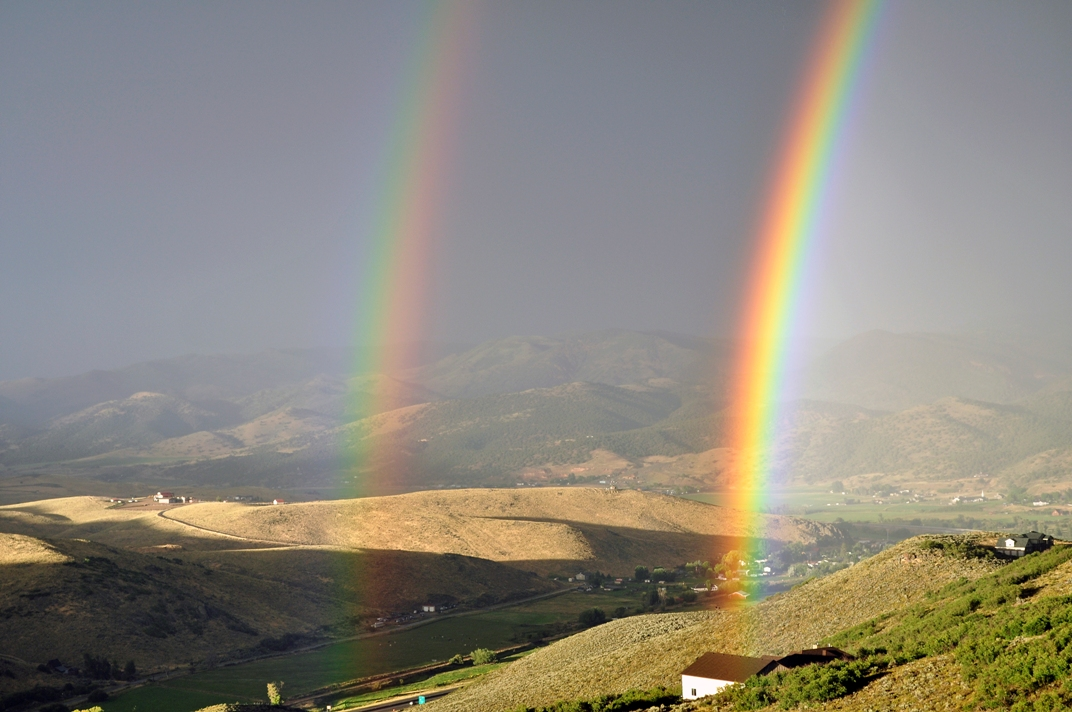
\includegraphics{images/doublerainbow.jpg}
\end{center}

\begin{itemize}
    \item Rainbows work through reflection and refraction of visible light on water drops. (insert image here)
    \item When the light refracts into the water drops, it reflects back and emerges out of the water drops, dispersing the light in the process.
    \item What about double rainbows? These are due to the secondary reflection from the light going into the water drops.
    \item If you're high up enough, sometimes you can see a circle rainbow \begin{center}
        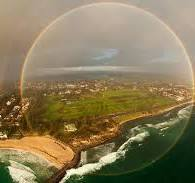
\includegraphics{images/circlerainbow.jpeg}
    \end{center}
\end{itemize}

\section*{Total Internal Reflection}

\begin{itemize}
    \item Snell's Law (again): \[n_{1}\sin{\theta_{1}} = n_{2}\sin{\theta_{2}}\]
    \item Critical angle of total internal reflection ray: \[\theta_{c} = \sin^{-1}{\Big(\frac{n_{2}}{n_{1}}\Big)}\]
    \item The critical angle for total internal reflection is the angle the light needs to travel at in order for it to be trapped by a material.
    \item \textbf{Fiber optics} are a great example of an application of total internal reflection. Light is put through the cables at a specific angle so that it keeps on internally reflecting through the cable to reach the other end.
\end{itemize}

\end{document}